\documentclass{article}
\usepackage[utf8]{inputenc}
\usepackage[T1]{fontenc}
\usepackage[english]{babel}
\usepackage{graphicx}
\usepackage{physics}
\usepackage{calrsfs}
\usepackage{mathalpha}
\usepackage{amssymb}
\usepackage{amsfonts}
\usepackage{amsmath}
\usepackage{fixltx2e}
\usepackage[dvipsnames]{xcolor}

\definecolor{myDarkGreen}{RGB}{0, 128, 0}


\title{2021-04-22 theory}
\author{}
\date{April 2021}

\begin{document}

\setcounter{section}{7}
\setcounter{subsection}{2}

\maketitle

\subsubsection{$Compression$ $\&$ $Merkle$-$Damg\ddot{a}rd$}
$Merkle$-$Damg\ddot{a}rd$ is a method to construct an \textbf{Hash} from a compression function \textbf{Com}. An \textit{IV} initialization vector is necessary.\\
\underline{After a padding}, the input $x$ is divided in blocks $x = x_1x_2x \dots x_n$ and it goes through the loop below:
\begin{center}
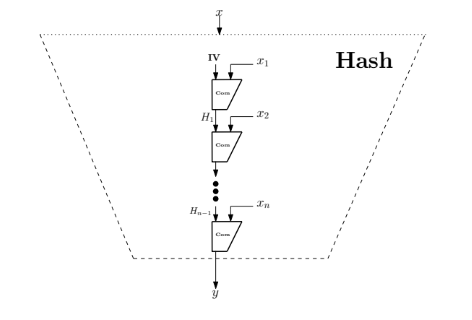
\includegraphics[]{Hash_Merkle-Damgard.png}
\end{center}
where each step $i$ is composed of an operation made by the compression function, which receive as input: 
\begin{itemize}
    \item a digest $H_{i-1}$ on $n$ bits (at first iteration it's the IV)
    \item the input block $x_i$ on $b$ bits ($b > n$)
\end{itemize}
and it outputs an hash $H_i$ on $n$ bits.\\
The final result is $y$: a compressed digest of the input $x$.\\ \\

The compression function can be implemented with a block cipher:\\
\textbf{\underline{Davies-Mayer construnction of $Com$ function}}\\
A block-cipher function $Enc$ is used to get a compression function $Com$:
\begin{center}
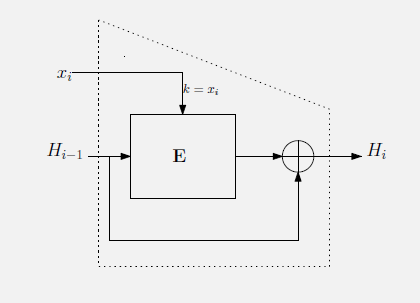
\includegraphics[]{Davis_Mayer.png}
\end{center}
Observe that the blocks $x_i$ are used as keys and the previous $H_i$'s as blocks to be ciphered.\\
\textcolor{myDarkGreen}{Notice the XOR at the end of the operation: \\
\begin{center}
$Enc_{x_i}(H_{i-1} \oplus H_{i-1})$
\end{center}
\\
By comparing it with Salsa20 and Chacha20, it is possible to notice that last XOR is used to implement a sort of key-whitening, as Salsa20 and Chacha20 do by inserting an additional ADD at the end of their iterations, in order to avoid recovering the key.
}\\

\underline{Exercise 7.2.4}:\textit{Show that David-Meyer function $Com$ has fixed points. Namely, for any $x_i$ there are $H$ such that: $H = Enc(H) \oplus H$}.\\

Solution:\\
A notable property of the Davies–Meyer construction is that even if the underlying block cipher is totally secure, it is possible to compute fixed points for the construction: for any $m$, one can find a value of $H$ such that $E_m(H) \oplus H = H$: one just has to set $H = E_m^{-1}(0)$. This is a property that random functions certainly do not have.

\vspace{5cm}

\underline{Exercise 7.2.5}:
\begin{center}
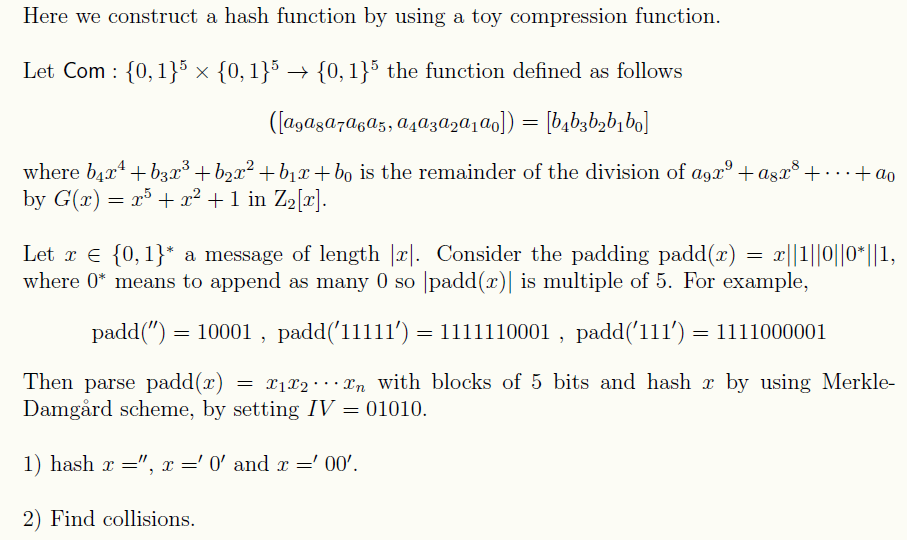
\includegraphics[width=130mm]{Exercise7_2_5.png}
\end{center}

Solution:\\
\begin{enumerate}
\item  a.   '' $\rightarrow$ padd('') = 10001 $\rightarrow$ Just 1 round: $H(x) = Enc(Iv, 10001) \oplus IV = Com(01010,10001)= 10110$  \\\\
       b.      '0' $\rightarrow$ padd('0') = 10001 $\rightarrow$ As  before.\\\\
       c.       '00' $\rightarrow$ padd('0') = 01001 $\rightarrow$ Just 1 round: $H = Enc(IV, 01001) \oplus IV = Com(01010,00101) = 00010$ \\\\
        
\item  The compression function can be written as $f: \{0,1\}^{2 \cdot 5} \rightarrow  \{0,1\}^{5}$. The hash function is not preimage resistant (it means that for a given $h$ in the output space of the hash function, it is not hard to find any message $x$ with $H(x)=h$). Since $f(H_{i-1}, m_i) = Enc_{H_{i-1}}(m_i)$ one can easily obtain a preimage of a single block message using the decryption function.
To obtain a second preimage or a collision, we use the same idea. Let $m=m_1 || m_2$ be a string of length $2 \cdot 5$ and we want another string with the same hash value. Let $H_0 = IV$, $H_1 = Enc_{IV}(m_1)$, $H_2 = Enc_{H_1}(m_2)$. That is $h = m_1 || m_2$ (note that we are already considering padding: "$m_i$" considers also padd() function).\\ Now choose $m'$ arbitrarily and set
\begin{center}
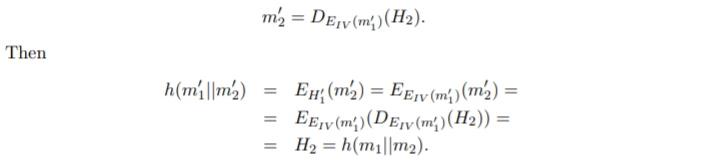
\includegraphics[width=130mm]{Exercise7_2_5_part2.png}
\end{center}
\end{enumerate}

\vspace{2cm}

\textbf{\underline{An example of $Merkle$-$Damg\ddot{a}rd$ application: RIPEMD-160}}\\ \\
RIPEMD-160 is a cryptographic hash function based upon the Merkle–Damgård construction. It is used in the Bitcoin standard in order to create a Bitcoin address. It is a a strengthened version of the RIPEMD algorithm which produces a 128 bit hash digest while the RIPEMD-160 algorithm produces a 160-bit output. The compression function is made up of 80 stages made up of 5 blocks that run 16 times each. This pattern runs twice with the results being combined at the bottom using modulo 32 addition.\\
The compression function is made up of a variable sub-block that the message block is passed though 16 times. There are 5 different variations for a total of 80 runs. This process occurs twice with the data meeting at the bottom to be moved on to the next block (if there is one) or added to the hash register is there isn't. The design of the sub-block and the overall layout of the compression function is shown below.\\ \\
\textit{RIPEMD-160 sub-block}:
\begin{center}
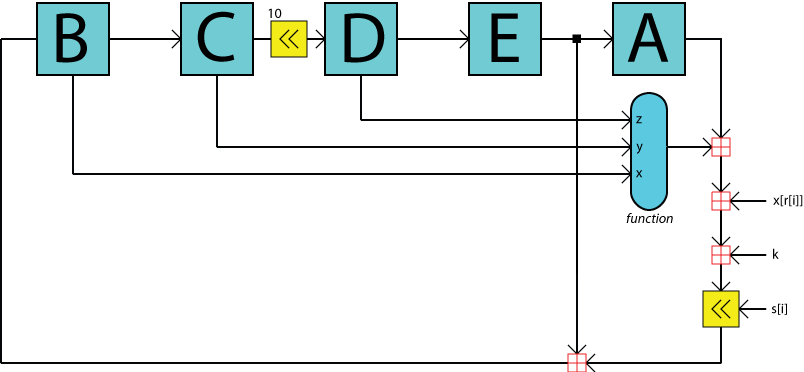
\includegraphics[width=100mm]{RIPEMD160_block.png}
\end{center}
Also elliptic curves are used to build a Bitcoin address.
\begin{flushleft}
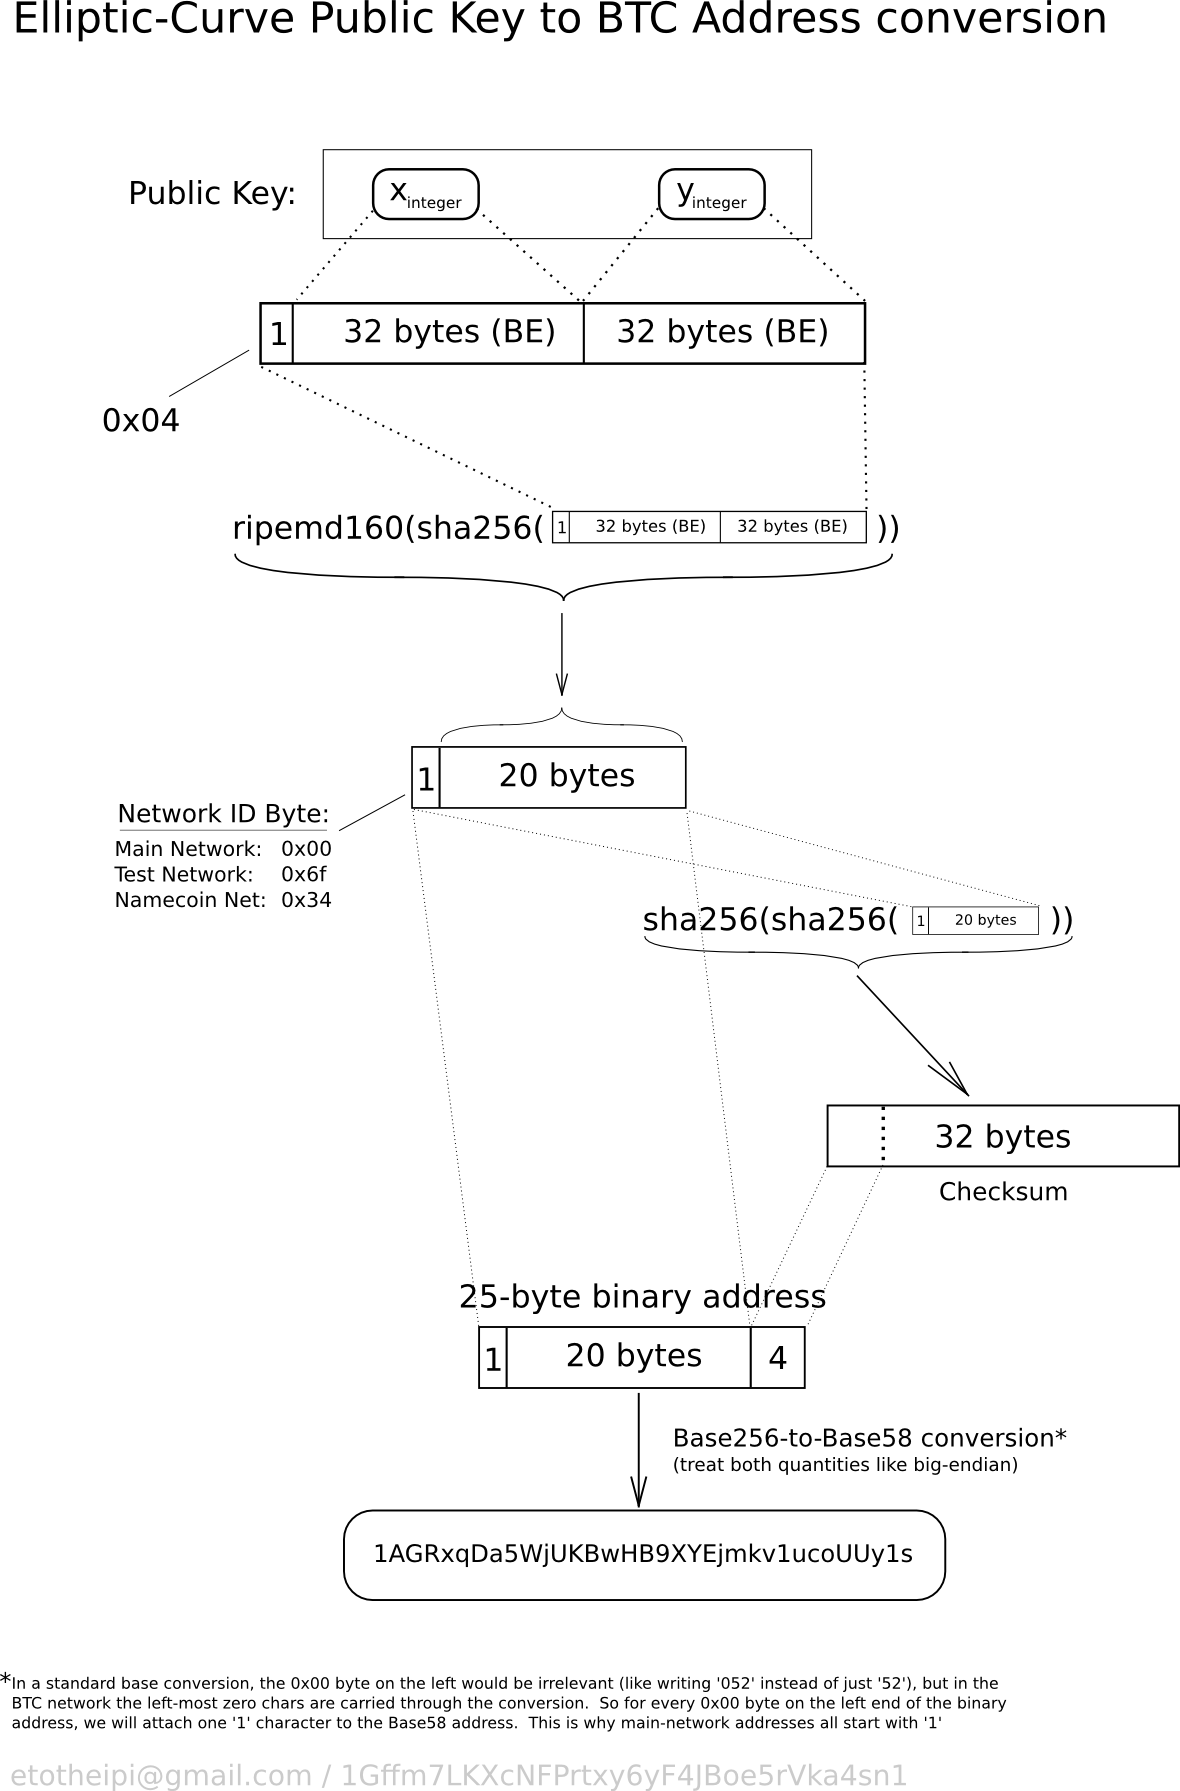
\includegraphics[width=160mm]{Bitcoin_PubKeyToAddr.png}
\end{flushleft}

\subsubsection{Hash via \underline{permutation}: Keccak Sponge and SHA3}

\textbf{History:}\\
In the past, SHA1 was used for cryptographic purposes but now it is deprecated since it is not secure: now it is used to compare files only (e.g. in GitHub). SHA2 family is still widely used but then, NIST organization chose SHA3 by means of a competition. A 1600 bits version of the Keccak algorithm was the winner of that competition. Examples of algorithms belonging to SHA3 family are:\\
\begin{itemize}
    \item SHA-3-512
    \item SHA-3-384
    \item SHA-3-256
    \item SHA-3-224
    \item etc.
\end{itemize}
where the last number is the digest bit length (not the security level!).\\
\underline{Note:} in SHA3 family there are also two extendable-output functions (XOFs) named SHAKE128 and SHAKE256 that are used to create a digest of a message of any desired length (in this case the number "128" or "256" indicates the security level (not the digest length). Example: SHAKE128$(msg, 333)$ outputs a 333 bits digest of the message $msg$.\\

SHA3 (Keccak) algorithm is based on a permutation function $f$:
\begin{center}
$f: \mathbb{Z}_{2}^{n} \rightarrow \mathbb{Z}_{2}^{n}$, $f$ biyective
\end{center}
$f$ should behave as a "Random Oracle": given an input register $x$, the function $f$ should generate $n$ random bits (computing $f(x)$ should be computationally feasible) and, if the same operation is repeated using the same input $x$, the result should be the same.\\

A sponge function or \textbf{sponge construction} is any of a class of algorithms with finite internal state that take an input bit stream of any length and produce an output bit stream of any desired length. A random sponge function is a sponge construction where $f$ is a random permutation, for example,  Keccak cryptographic sponge with a 1600-bit state ($f$ could be any kind of permutation function).\\
SHA-3 uses the sponge construction, in which data is "absorbed" into the sponge, then the result is "squeezed" out. In the absorbing phase, message blocks are XORed into a subset of the state, which is then transformed as a whole using a permutation function $f$. In the "squeeze" phase, output blocks are read from the same subset of the state, alternated with the state transformation function $f$. The size of the part of the state that is written and read is called the "rate" (denoted $r$), and the size of the part that is untouched by input/output is called the "capacity" (denoted $c$). The capacity determines the security of the scheme. The maximum security level is half the capacity ($\frac{c}{2}$) since it requires a loop of $2^{\frac{c}{2}}$ iterations.\\

\begin{center}
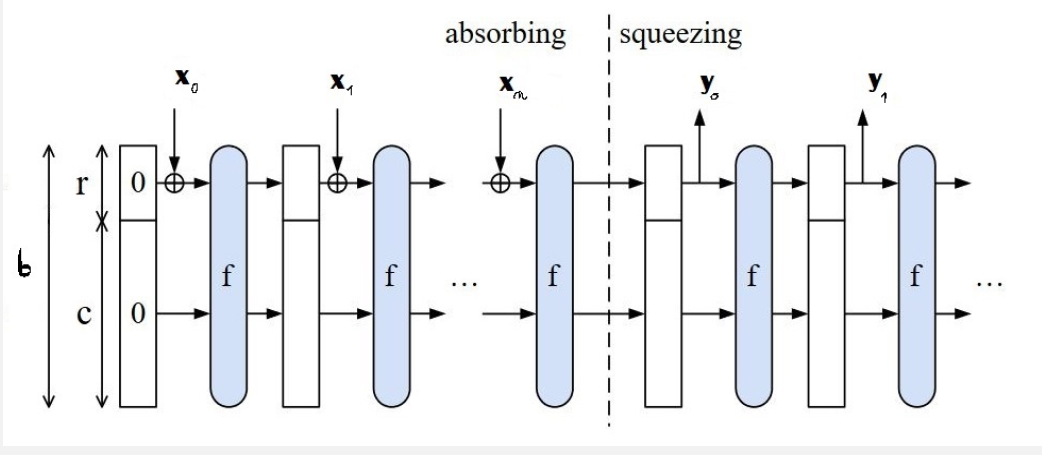
\includegraphics[width=130mm]{sponge_construction.png}
\end{center}

Input $x$ is divided in blocks $x_i$ of $r$ bits (a padding is included). The number $b$ is called "width", sum of the capacity and the bitrate. The state of the sponge is the content of a register of $b$ bits, while $f$ is the permutation of the state, i.e. a $\mathbb{Z}_{2}^{b}$.\\
The two phases are:
\begin{enumerate}
    \item \textcolor{red}{absorbing}: the input $r$-bits of block $x_i$ are XORed with the $r$ bits of the state. Then $f$ is used to permute the state. This is done until all blocks are "absorbed".
    \item \textcolor{red}{squeezing}: the output is computed as $y=y_0||y_1|| \cdots$ by using the $r$ bits $y_i$ of the state.
\end{enumerate}
The last $c$ bits of the state are not altered by the blocks $x_i$ and they are NOT part of the output.\\

In SHA-3 Keccak permutation function $f$, each round consists of a sequence of five steps denoted by Greek letters: $\theta$ (theta), $\rho$ (rho), $\pi$ (pi), $\chi$ (chi) and $\iota$ (iota). Each step manipulates the entire state.\\

Keccak permutation function $f$ is invertible so, if the entire register is output, then the procedure will be reversible: this is why only part of it is taken as output at each squeezing step.
The capacity determines the claimed level of security, and one can trade claimed security for speed by increasing the capacity $c$ and decreasing the bitrate $r$ accordingly, or viceversa.\\

- Example (SHA3): \\
\indent \indent $b=1600$, so $r$ could be: 1152, 1088, 832, 576, ...\\

Comparison between generic Keccak algorithm and SHA3:\\
\begin{itemize}
    \item Keccak (also called Keccak-f[b]):\\
           - $b$ can be freely chosen.\\
           - Padding is computed as M||10*1 ('1' and '0' are defined bits, while '*' indicates that there is a variable string of 0 bits that depends on value of $r$).\\
           - Once $b$ is chosen, then the number of rounds used for computation is known (example: $b=25 \Rightarrow 12$ rounds [see Section 2 for more details: there's the construction of a keystream by means of Keccak, not of an hash, but the function is the same], since $b=25 \cdot 2^l$ and so there will be $12+2l$ rounds (12 rounds for $l$=0). 
    \item SHA3:\\
           - $b$ is fixed ($b$=1600).\\
           - Padding is different: M||0110*1\\
           - In this case there are 24 rounds for $b=1600$ and $l=6$: in fact $12+2 \cdot 6 = 24$.\\
\end{itemize}

\underline{Exercise 7.2.6}:\\
\textit{The permutation $f$ is not required to be one-way. So why hashing with a sponge should be preimage resistant? Assume that r = 512, b = 1600 and that after padding your message $M$ is $x_0$. So the hash digest is $y_0$. Write a loop to find a second preimage of $y_0$. How many
cycles are expected?}

\textit{\underline{Premise:} A public function H from set $A$ to finite set $B$ is: \begin{itemize}
    \item first-preimage-resistant when for a given random $b$ in $B$, it is hard to exhibit a preimage of $b$, that is, $a$ in $A$ with $H(a)=b$.
    \item Second-preimage-resistant when for a given random $a_0$ in $A$, it is hard to exhibit another preimage of $b=H(a_0)$, that is, $a$ in $A$ with $a \neq a_0$ and $H(a)=H(a_0)$ (in other words: Given a \textbf{fixed} input $m_1$ it should be difficult to find another input $m_2$ such that $m_1 \neq m_2$ and hash($m_1$)=hash($m_2$). Functions that lack this property are vulnerable to second-preimage attacks)
    \item Collision-resistant: like second-preimage-resistant but $m_1$ and $m_2$ can be both freely chosen by the attacker.
\end{itemize}
A preimage can in principle be found by trying various values of $a$ in $A$ (other that $a_0$ for second-preimage), and computing $H(a)$ until it matches $b$.}\\

By definition, an ideal hash function is such that the fastest way to compute a first or second preimage is through a brute-force attack. For an n-bit hash, this attack has a time complexity $2^n$, which is considered too high for a typical output size of $n$ = 128 bits. If such complexity is the best that can be achieved by an adversary, then the hash function is considered preimage-resistant. However, there is a general result that quantum computers perform a structured preimage attack in $\sqrt{2^n} = 2n/2$, which also implies second preimage.\\

"An iterated function, like this Keccak sponge, uses a finite memory to store its state and processes the input, block per block. At any point in time, the state of the iterated function summarizes the input blocks received so far. Because it contains a finite number of bits, collisions can happen in this state. Random oracles, on the other hand, do not have collisions in their state as such a concept does not exist. This is the main reason for which random oracles cannot be used directly to express security claims of functions with variable-length output: they would simply never exhibit any effects of the finite memory any concrete iterated function has.
Random sponges functions, on the other hand, provide an alternative to the random oracle model for expressing security claims. A random sponge is an instance of the sponge construction with $f$ chosen randomly from the set of transformations (or of permutations) over $b$ bits. We have proven that a random sponge function is as strong as a random oracle, except for the effects induced by the finite memory. A random sponge can serve as a reference model for expressing compact security claims for iterated hash functions and stream ciphers." $\sim$ \textit{Keccak team}\\

\underline{Solution:}
This exercise is about the first step of the sponge \textbf{only}. So, to solve this exercise, it is enough to perform a brute force loop: find another $x_0$ such that the output is again $y_0$ (the $c$ bits of the final register can be dropped out).
\begin{center}
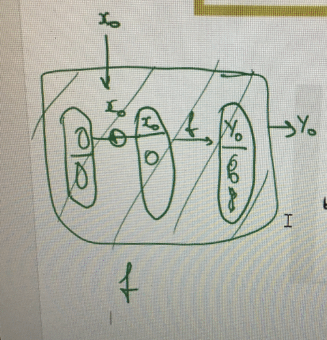
\includegraphics[width=70mm]{Exercise7_2_6.png}\\
\end{center}



\underline{Exercise 7.2.7}:\\
\begin{center}
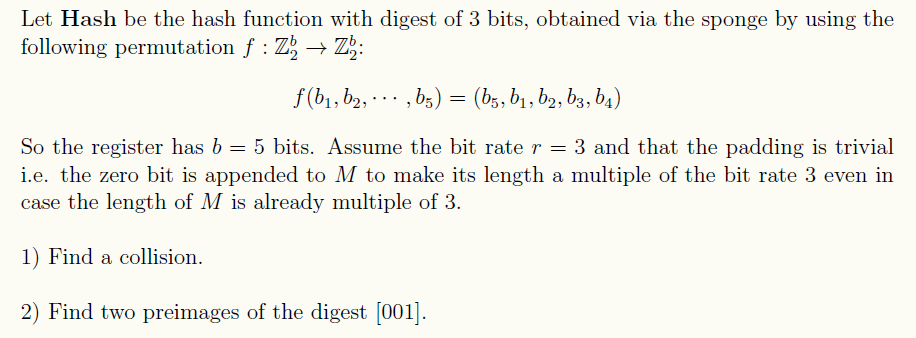
\includegraphics[width=130mm]{Exercise7_2_7.png}
\end{center}

1) See point '2)'.\\

2) In order to obtain [001] as digest and assuming that the input message is only 3 bits long (no padding and no division in blocks are needed) it is necessary to have a register such that the reversed permutation leads to:\\
       \begin{center}
       [01xx0]  $\leftarrow$  [001xx]\\
       \end{center}
So, in order to obtain [01xx0], we need to reverse the XOR operation made with the input $x_0$:\\
       \begin{center}
       [000 00] $\oplus$ [ttt 00] = [01x 00]   $\rightarrow$   [01xx0]\\
       \end{center}
In the end, we have to find the three bits 'ttt', knowing that, XORed with '000' must give the '01x' outcome. There are two possible solutions (the two preimages):\\
    - [000] $\oplus$ \textcolor{myDarkGreen}{[010]} = [010]\\
    - [000] $\oplus$ \textcolor{myDarkGreen}{[011]} = [011]\\
    
\vspace{5cm}

\underline{Exercise 7.2.8}:
\begin{center}
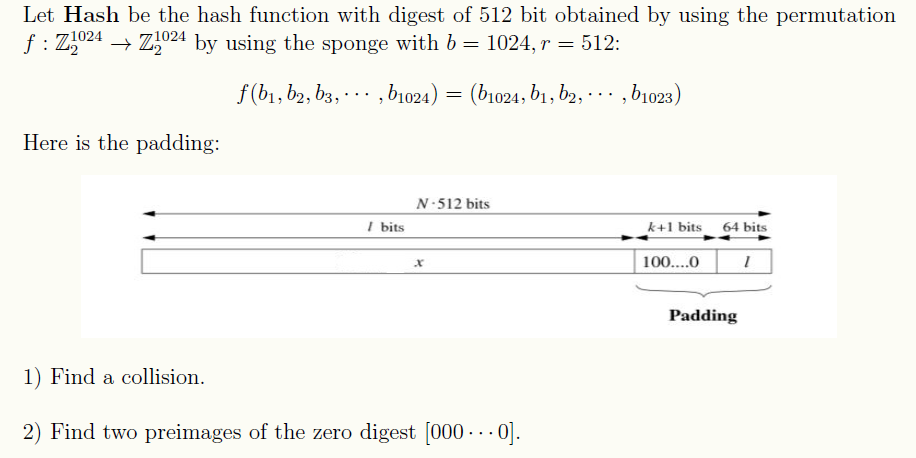
\includegraphics[width=130mm]{Exercise7_2_8.png}
\end{center}

Solution of this exercise is the same as the previous one, but since the register size is much greater, a coding implementation is needed to perform the operations.\\

\subsection{Bit Commitment}

\begin{center}
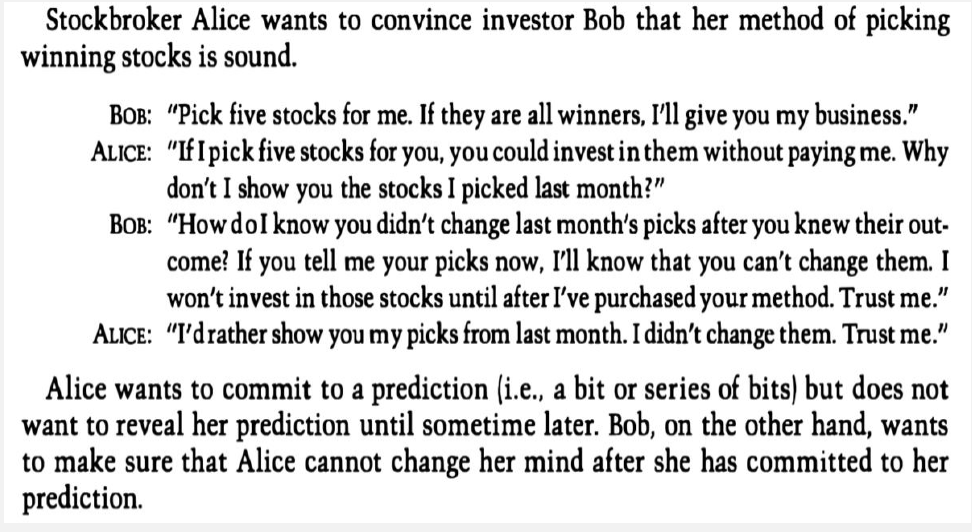
\includegraphics[width=130mm]{bitcommitment_intro.png}
\end{center}

A commitment scheme is a protocol for Alice and Bob with two different phases and algorithm $Com$ (\textcolor{orange}{Warning:} here it is NOT $Com$="Compression", it is $Com$="Commitment").
\begin{itemize}
    \item Commitment phase: Alice has a secret $b$ to commit and sends to Bob a commitment value $c$ (commitment for $b$). The value $c$ is the output $c=Com(b,r)$ of the algorithm $Com$; $r$ indicates that $c$ is computed by $b$ and some random value $r$. 
    \item Opening/Reveal phase: Alice sends to Bob the former secret $b$ so Bob can check if $c'=Com(b,r)$ for $r$ is equal to $c$ ($r$ is pre-shared among Alice and Bob, so Bob knows $r$).
\end{itemize}
A commitment scheme is secure if these two properties are satisfied:
\begin{enumerate}
    \item Hiding property: at the end of the first phase, Bob (even dishonest) does not has any information about $b$.
    \item Binding property: for a given $c$, there is an unique value of $b$ that convince Bob, so Alice (even dishonest) cannot choose another $b$. 
\end{enumerate}

An application of this scheme is shown in the next exercise:\\ \\
\underline{Exercise 7.3.1}: Cryptographic coin flipping\\
\textit{By using a commitment scheme for a single bit ($b \in \{0, 1\}$)
construct a protocol for the problem of “flipping a coin by telephone”. That is to say, Alice and Bob want to flip a coin by telephone. (They have just divorced, live in different cities, want to decide who gets the car.) Bob would not like to tell Alice HEADS and hear Alice (at the other end of the line) saying “Here goes...I’m flipping the coin... You lost !”
Hint: start with some naive protocol e.g. Alice chooses a random bit $b_A$ and send it to Bob. Bob does the same and chooses a random bit $b_B$ and send it to Alice. The output bit for both is $b=b_A \oplus b_B$.}\\

Alice and Bob can use commitments in a procedure that will allow both to trust the outcome:\\
\begin{itemize}
    \item Alice "calls" the coin flip but only tells Bob a commitment to her call ($c_A = Com(b_A, r_A)$, $c_A$ sent to Bob)
    \item Bob flips the coin and reports the result  ($c_B = Com(b_B, r_B)$, $c_B$ sent to Alice)
    \item Alice reveals what she committed to ($b_A$ and $r_A$ are sent to Bob)
    \item Bob verifies that Alice's call matches her commitment ($c'= Com(b_A, r_A) \rightarrow c' == c_A ?$)
    \item If Alice's revelation matches the coin result Bob reported, Alice wins
\end{itemize}
For Bob to be able to skew the results to his favor, he must be able to understand the call hidden in Alice's commitment. If the commitment scheme is a good one, Bob cannot skew the results. Similarly, Alice cannot affect the result if she cannot change the value she commits to.\\

\underline{Exercise 7.3.2}:\\
\textit{Construct a commitment algorithm Com by using a Hash random oracle.}\\

Bit-commitment schemes are trivial to construct in the random oracle model. Given a hash function $H$ with a 3$k$ bit output, to commit the $k$-bit message $m$, Alice generates a random $k$ bit string $R$ and sends Bob $H(R||m)$. The probability that any $R'$, $m'$ exist where $m' \neq m$ such that $H(R'||m') = H(R||m)$ is $\approx 2−k$, but to test any guess at the message $m$ Bob will need to make $2k$ (for an incorrect guess) or $2k-1$ (on average, for a correct guess) queries to the random oracle. We note that earlier schemes based on hash functions, essentially can be thought of schemes based on idealization of these hash functions as random oracle.

\subsection{MAC: Message Authentication Code}
A MAC is a \underline{symmetric} algorithm that allows to check the authenticity of the message.\\

A MAC consists of three algorithms:
\begin{itemize}
    \item $Gen(n)$: the input $n$ is a security parameter and the output is a key $k$ of $n$ bits (\textit{key-generation}). To perform this phase the starting point could be an hash but you must be careful since it could lead to an attack (see later: subsection 7.4.1).
    \item $Mac_k(m)$: inputs are a message $m$ and a key $k$. The output is a tag $t$ (\textit{tag-generation}).
    \item Vrfy$_k(m)$: inputs are a message $m$, a key $k$ and a tag $t$. Output is 1 for "valid tag" or 0 for "invalid tag" (\textit{verification}). 
\end{itemize}
A MAC is secure if an adversary who does not know $k$, but knows some valid tags
$(m_1, t_1) \cdots (m_l, t_l)$, it is not able to produce a valid pair $(m, t)$ where $t$ is a valid tag for the message $m$, with of course $m \neq m_i$, $\forall i$.\\

\vspace{5cm}

\underline{Exercise 7.4.2}:
\begin{center}
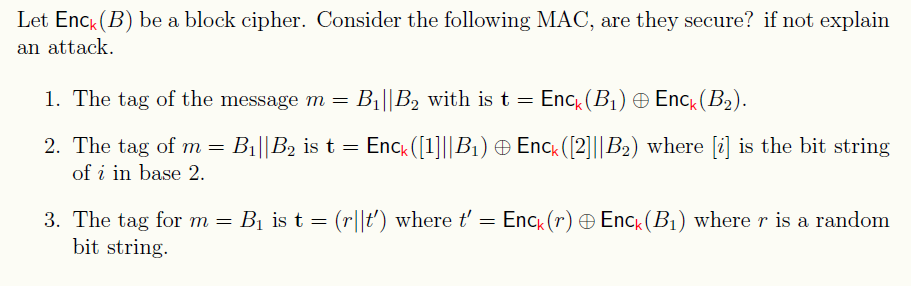
\includegraphics[width=130mm]{Exercise7_4_2.png}
\end{center}

\begin{enumerate}
    \item In this case, all the messages like $B_i||B_i$ have the same tag $t=[0]$. So, an adversary already knows a lot of combinations.
    \item In this case an adversary in CPA scenario can ask to oracle tag of these messages: $B_1||B_2$, $B_1'||B_2 and B_1||B_2', so by doing the XOR it will obtain:$
    \begin{center}
    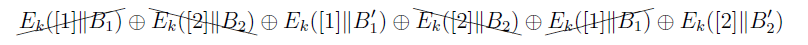
\includegraphics[width=130mm]{ex_espression.png}
    \end{center}
    So it has obtained the tag of message $B_1'||B_2'$,, different from previous three.
    \item In this case, if PNRG is secure, also MAC is secure.
\end{enumerate}


\subsubsection{Attack: Length extensions \& HMAC}
\textit{This is an attack to the MAC constructed from the hash, not directly to the hash.}\\

A naive way to get a MAC is by using a hash function: given $k$ and $P$ a tag for the message $P$ is just $t = Hash(k||P)$.\\

The attack consists in:
\begin{center}
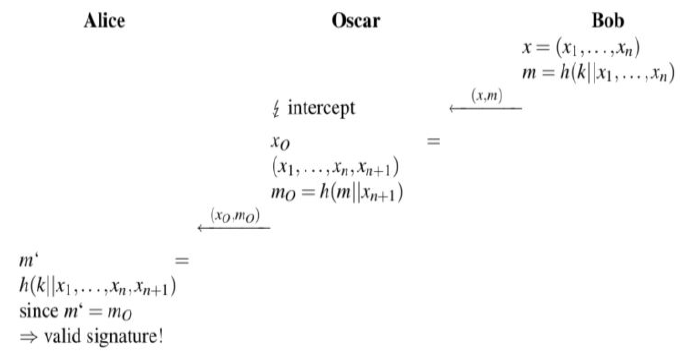
\includegraphics[width=130mm]{MAC_attack.png}
\end{center}

So the above naive MAC it is not secure if the Hash is designed with the $Merkle$-$Damg\ddot{a}rd$ method. This is a special case of a more general Lenght extension attack.
This design problem of a Hash is fixed by using HMAC.\\

\textbf{HMAC}:\\
A Hash-based Message Authentication Code which does not show the security weakness described above is the HMAC construction, proposed in 1996. The scheme consists of an inner and outer hash.
\begin{center}
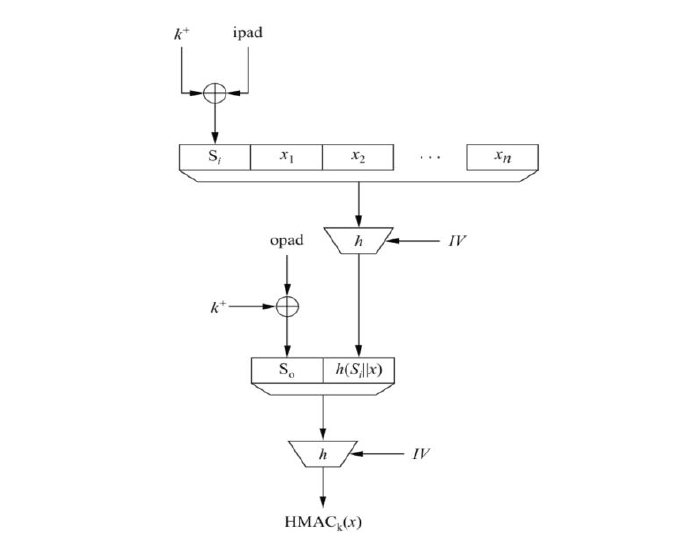
\includegraphics[width=110mm]{hmac.png}
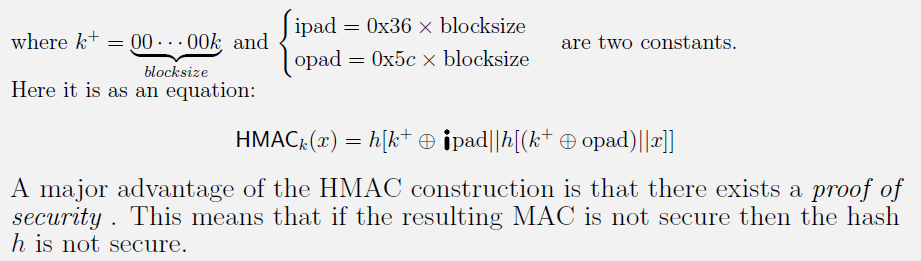
\includegraphics[width=130mm]{hmac2.png}
\end{center}


\end{document}
